% ===========================================================================
%  TikuOS — TikuKits DS: Queue for Embedded Systems
%  Beamer Presentation
% ===========================================================================
\documentclass[aspectratio=169, 10pt]{beamer}

% ---- Theme ----------------------------------------------------------------
\usetheme{Madrid}
\usecolortheme{whale}
\setbeamertemplate{navigation symbols}{}
\setbeamertemplate{footline}{%
  \leavevmode\hbox{%
    \begin{beamercolorbox}[wd=.33\paperwidth,ht=2.5ex,dp=1ex,center]{author in head/foot}%
      \usebeamerfont{author in head/foot}\insertshortauthor
    \end{beamercolorbox}%
    \begin{beamercolorbox}[wd=.34\paperwidth,ht=2.5ex,dp=1ex,center]{title in head/foot}%
      \usebeamerfont{title in head/foot}\insertshorttitle
    \end{beamercolorbox}%
    \begin{beamercolorbox}[wd=.33\paperwidth,ht=2.5ex,dp=1ex,right]{date in head/foot}%
      \usebeamerfont{date in head/foot}\insertshortdate{}\hspace*{2em}%
      \insertframenumber{}/\inserttotalframenumber\hspace*{2ex}
    \end{beamercolorbox}}%
  \vskip0pt%
}

% ---- Packages -------------------------------------------------------------
\usepackage{listings}
\usepackage{graphicx}
\usepackage{hyperref}
\usepackage{booktabs}
\usepackage{multirow}
\usepackage{tikz}
\usetikzlibrary{arrows.meta, positioning, shapes.geometric, calc,
                decorations.pathreplacing, fit}
\usepackage{amsmath}

% ---- Code listing style ---------------------------------------------------
\lstset{
  basicstyle=\ttfamily\scriptsize,
  keywordstyle=\color{blue}\bfseries,
  commentstyle=\color{gray},
  stringstyle=\color{red!70!black},
  showstringspaces=false,
  breaklines=true,
  frame=single,
  rulecolor=\color{black!30},
  backgroundcolor=\color{blue!3},
  tabsize=4,
}
\lstdefinestyle{cstyle}{
  language=C,
  morekeywords={uint8_t,uint16_t,uint32_t,int32_t,int16_t,
                tiku_kits_ds_elem_t,
                TIKU_KITS_DS_OK,TIKU_KITS_DS_ERR_NULL,
                TIKU_KITS_DS_ERR_FULL,TIKU_KITS_DS_ERR_EMPTY,
                TIKU_KITS_DS_ERR_PARAM,TIKU_KITS_DS_ERR_NOTFOUND,
                TIKU_KITS_DS_ERR_BOUNDS,
                TIKU_KITS_DS_QUEUE_MAX_SIZE,
                NULL},
}

% ---- Metadata -------------------------------------------------------------
\title[TikuKits DS]{TikuKits DS: Queue for Embedded Systems}
\subtitle{Simple. Ubiquitous. Intelligence, Everywhere.}
\author[Ambuj Varshney]{Ambuj Varshney \\ \texttt{ambuj@tiku-os.org}}
\date{\today}

% ===========================================================================
\begin{document}

% ---------------------------------------------------------------------------
\begin{frame}
\titlepage
\end{frame}

% ---------------------------------------------------------------------------
\begin{frame}{Outline}
\tableofcontents
\end{frame}

% ===========================================================================
\section{Motivation}
% ===========================================================================

\begin{frame}{Why a Queue on MCUs?}
\begin{columns}[T]
\begin{column}{0.48\textwidth}
\begin{block}{Embedded Use Cases}
\begin{itemize}
  \item \textbf{Event queue} --- ISR posts events, main loop processes
  \item \textbf{Command buffer} --- queue commands for sequential execution
  \item \textbf{Message passing} --- inter-process or task-to-task communication
  \item \textbf{Print/log queue} --- buffer debug output for deferred printing
  \item \textbf{Task scheduling} --- fair round-robin ordering
\end{itemize}
\end{block}

\begin{block}{Constraints}
\begin{itemize}
  \item No heap allocation
  \item Fixed, bounded memory usage
  \item $O(1)$ enqueue and dequeue
  \item FIFO ordering guarantee
\end{itemize}
\end{block}
\end{column}

\begin{column}{0.48\textwidth}
\begin{center}
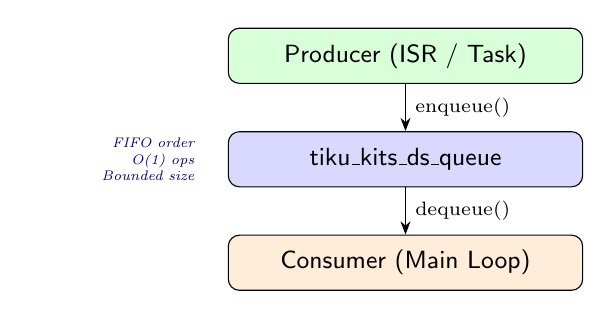
\begin{tikzpicture}[
    >=Stealth, node distance=0.5cm
  ]
  \node[draw, rounded corners, minimum height=0.7cm,
        text centered, font=\small\sffamily, fill=green!15,
        minimum width=4.5cm] (prod) {Producer (ISR / Task)};
  \node[draw, rounded corners, minimum height=0.7cm,
        text centered, font=\small\sffamily, fill=blue!15,
        minimum width=4.5cm, below=0.6cm of prod] (q)
    {tiku\_kits\_ds\_queue};
  \node[draw, rounded corners, minimum height=0.7cm,
        text centered, font=\small\sffamily, fill=orange!15,
        minimum width=4.5cm, below=0.6cm of q] (cons)
    {Consumer (Main Loop)};
  \draw[->] (prod) -- node[right, font=\scriptsize] {enqueue()} (q);
  \draw[->] (q) -- node[right, font=\scriptsize] {dequeue()} (cons);

  \node[left=0.3cm of q, font=\tiny\itshape, text=blue!50!black,
        text width=2cm, align=right] {FIFO order\\O(1) ops\\Bounded size};
\end{tikzpicture}
\end{center}

\vspace{0.5em}
\begin{alertblock}{Design Goal}
Provide a fixed-size FIFO queue with $O(1)$ enqueue/dequeue,
\textbf{zero heap usage}, and clear semantic naming
(\texttt{enqueue}/\texttt{dequeue}) for application-level use.
\end{alertblock}
\end{column}
\end{columns}
\end{frame}

% ===========================================================================
\section{Queue vs. Ring Buffer}
% ===========================================================================

\begin{frame}{Queue vs. Ring Buffer: What is the Difference?}
\begin{columns}[T]
\begin{column}{0.48\textwidth}
\begin{block}{Ring Buffer (\texttt{ringbuf})}
\begin{itemize}
  \item \textbf{Low-level primitive} for circular storage
  \item API: \texttt{push} / \texttt{pop} / \texttt{peek}
  \item Typically used as a byte-level or sample-level buffer
  \item Consumer may also be a producer (bidirectional patterns)
  \item Used by: UART drivers, DMA buffers, signal pipelines
\end{itemize}
\end{block}
\end{column}

\begin{column}{0.48\textwidth}
\begin{block}{Queue (\texttt{queue})}
\begin{itemize}
  \item \textbf{Application-level FIFO} abstraction
  \item API: \texttt{enqueue} / \texttt{dequeue} / \texttt{peek}
  \item Represents a logical queue of items (events, commands, messages)
  \item Strict producer--consumer discipline
  \item Used by: event dispatchers, command processors, schedulers
\end{itemize}
\end{block}
\end{column}
\end{columns}

\vspace{0.5em}
\begin{alertblock}{Same Mechanism, Different Abstraction}
Both are implemented with circular-buffer arithmetic internally.
The \textbf{queue} module provides domain-specific naming
(\texttt{enqueue}/\texttt{dequeue}) and a smaller default capacity (16 vs.\ 32)
suited for event-driven embedded applications. Choose the abstraction
that matches your intent.
\end{alertblock}
\end{frame}

% ===========================================================================
\section{Data Structure}
% ===========================================================================

\begin{frame}[fragile]{The \texttt{tiku\_kits\_ds\_queue} Structure}
\begin{columns}[T]
\begin{column}{0.48\textwidth}
\begin{lstlisting}[style=cstyle,
  title={ds/queue/tiku\_kits\_ds\_queue.h}]
#ifndef TIKU_KITS_DS_QUEUE_MAX_SIZE
#define TIKU_KITS_DS_QUEUE_MAX_SIZE 16
#endif

struct tiku_kits_ds_queue {
    tiku_kits_ds_elem_t
        data[TIKU_KITS_DS_QUEUE_MAX_SIZE];
    uint16_t head;      /* dequeue index */
    uint16_t tail;      /* enqueue index */
    uint16_t count;     /* valid elements */
    uint16_t capacity;  /* user limit    */
};
\end{lstlisting}

\vspace{0.3em}
\textbf{Memory footprint:}\\
$16 \times 4 + 4 \times 2 = 72$ bytes (default).\\
All statically allocated --- no heap.
\end{column}

\begin{column}{0.48\textwidth}
\textbf{FIFO flow:}
\begin{center}
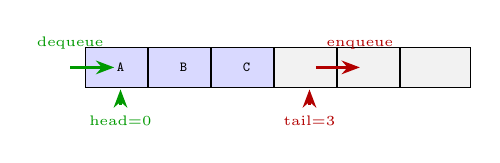
\begin{tikzpicture}[>=Stealth, scale=0.8]
  % Queue slots (horizontal)
  \foreach \i/\v in {0/A, 1/B, 2/C, 3/{}, 4/{}, 5/{}} {
    \pgfmathsetmacro{\fillcol}{\i < 3 ? "blue!15" : "gray!10"}
    \node[draw, minimum width=0.9cm, minimum height=0.5cm,
          fill=\fillcol, font=\tiny\ttfamily] (s\i) at (\i*1.0, 0) {\v};
  }

  % Head and tail markers
  \draw[->, thick, green!60!black] (0, -0.6) -- (0, -0.35)
    node[below=0.2cm, font=\tiny] {head=0};
  \draw[->, thick, red!70!black] (3*1.0, -0.6) -- (3*1.0, -0.35)
    node[below=0.2cm, font=\tiny] {tail=3};

  % Arrows
  \draw[->, thick, green!60!black] (-0.8, 0) -- (-0.1, 0)
    node[above=0.1cm, font=\tiny, pos=0] {dequeue};
  \draw[->, thick, red!70!black] (3.1*1.0, 0) -- (3.8*1.0, 0)
    node[above=0.1cm, font=\tiny, pos=1] {enqueue};
\end{tikzpicture}
\end{center}

\vspace{0.5em}
\begin{block}{Key Properties}
\begin{itemize}
  \item \texttt{head}: index of next element to dequeue
  \item \texttt{tail}: index of next free slot for enqueue
  \item \texttt{count}: distinguishes full from empty
  \item Modulo wrap: \texttt{(idx + 1) \% capacity}
\end{itemize}
\end{block}
\end{column}
\end{columns}
\end{frame}

% ===========================================================================
\section{API Reference}
% ===========================================================================

\begin{frame}[fragile]{Complete API}
\begin{table}
\centering
\small
\begin{tabular}{@{}lp{8cm}@{}}
\toprule
\textbf{Function} & \textbf{Description} \\
\midrule
\texttt{\_queue\_init(q, cap)}
  & Initialize with capacity $1 \ldots$ \texttt{MAX\_SIZE}; zeros data \\
\texttt{\_queue\_enqueue(q, val)}
  & Add element at tail, advance tail; returns \texttt{ERR\_FULL} \\
\texttt{\_queue\_dequeue(q, \&val)}
  & Remove element from head, advance head; returns \texttt{ERR\_EMPTY} \\
\texttt{\_queue\_peek(q, \&val)}
  & Read head element without removing \\
\midrule
\texttt{\_queue\_clear(q)}
  & Reset head, tail, count to 0 \\
\texttt{\_queue\_size(q)}
  & Return current number of elements \\
\texttt{\_queue\_full(q)}
  & Return 1 if count $=$ capacity \\
\texttt{\_queue\_empty(q)}
  & Return 1 if count $= 0$ \\
\bottomrule
\end{tabular}
\end{table}

\vspace{0.3em}
{\scriptsize All functions are prefixed with \texttt{tiku\_kits\_ds}.
Every function validates pointer arguments and returns \texttt{ERR\_NULL} on failure.}

\begin{alertblock}{FIFO Guarantee}
\texttt{dequeue()} always returns the element that was \texttt{enqueue()}'d
earliest --- strict first-in, first-out ordering is maintained even through
index wraparound.
\end{alertblock}
\end{frame}

% ===========================================================================
\section{How It Works}
% ===========================================================================

\begin{frame}[fragile]{Enqueue and Dequeue Implementation}
\begin{columns}[T]
\begin{column}{0.48\textwidth}
\begin{lstlisting}[style=cstyle,
  title={enqueue --- write at tail, wrap}]
int tiku_kits_ds_queue_enqueue(
    struct tiku_kits_ds_queue *q,
    tiku_kits_ds_elem_t value)
{
    if (q == NULL)
        return TIKU_KITS_DS_ERR_NULL;
    if (q->count >= q->capacity)
        return TIKU_KITS_DS_ERR_FULL;

    q->data[q->tail] = value;
    q->tail = (q->tail + 1)
              % q->capacity;
    q->count++;
    return TIKU_KITS_DS_OK;
}
\end{lstlisting}
\end{column}

\begin{column}{0.48\textwidth}
\begin{lstlisting}[style=cstyle,
  title={dequeue --- read from head, wrap}]
int tiku_kits_ds_queue_dequeue(
    struct tiku_kits_ds_queue *q,
    tiku_kits_ds_elem_t *value)
{
    if (q == NULL || value == NULL)
        return TIKU_KITS_DS_ERR_NULL;
    if (q->count == 0)
        return TIKU_KITS_DS_ERR_EMPTY;

    *value = q->data[q->head];
    q->head = (q->head + 1)
              % q->capacity;
    q->count--;
    return TIKU_KITS_DS_OK;
}
\end{lstlisting}
\end{column}
\end{columns}

\vspace{0.3em}
\begin{block}{Identical to Ring Buffer Internals}
The circular-buffer mechanism is the same: modulo wrap on head and tail,
count field for occupancy. The difference is purely in the API naming
(\texttt{enqueue}/\texttt{dequeue} vs.\ \texttt{push}/\texttt{pop}) and
the intended abstraction level.
\end{block}
\end{frame}

% ===========================================================================
\section{Code Examples}
% ===========================================================================

\begin{frame}[fragile]{Example 1: Basic Enqueue, Dequeue, and Peek}
\begin{lstlisting}[style=cstyle,
  title={Basic queue usage}]
#include "tikukits/ds/queue/tiku_kits_ds_queue.h"

struct tiku_kits_ds_queue q;
tiku_kits_ds_elem_t val;

/* Initialize with capacity 8 */
tiku_kits_ds_queue_init(&q, 8);

/* Enqueue three events */
tiku_kits_ds_queue_enqueue(&q, 100);   /* event A */
tiku_kits_ds_queue_enqueue(&q, 200);   /* event B */
tiku_kits_ds_queue_enqueue(&q, 300);   /* event C */

/* Peek: see the next event without consuming it */
tiku_kits_ds_queue_peek(&q, &val);     /* val == 100 */

/* Dequeue: FIFO order */
tiku_kits_ds_queue_dequeue(&q, &val);  /* val == 100 */
tiku_kits_ds_queue_dequeue(&q, &val);  /* val == 200 */
tiku_kits_ds_queue_dequeue(&q, &val);  /* val == 300 */

/* Queue is now empty */
int rc = tiku_kits_ds_queue_dequeue(&q, &val);
/* rc == TIKU_KITS_DS_ERR_EMPTY */
\end{lstlisting}
\end{frame}

% ---------------------------------------------------------------------------
\begin{frame}[fragile]{Example 2: Wraparound Behavior}
\begin{columns}[T]
\begin{column}{0.48\textwidth}
\begin{lstlisting}[style=cstyle,
  title={Fill, drain partially, refill}]
struct tiku_kits_ds_queue q;
tiku_kits_ds_elem_t val;

tiku_kits_ds_queue_init(&q, 4);

/* Fill: [10, 20, 30, 40] */
tiku_kits_ds_queue_enqueue(&q, 10);
tiku_kits_ds_queue_enqueue(&q, 20);
tiku_kits_ds_queue_enqueue(&q, 30);
tiku_kits_ds_queue_enqueue(&q, 40);
/* full: head=0, tail=0, count=4 */

/* Dequeue two */
tiku_kits_ds_queue_dequeue(&q, &val);
/* val=10, head=1 */
tiku_kits_ds_queue_dequeue(&q, &val);
/* val=20, head=2 */

/* Enqueue two more: tail wraps */
tiku_kits_ds_queue_enqueue(&q, 50);
tiku_kits_ds_queue_enqueue(&q, 60);
/* full again: count=4 */

/* Dequeue all: 30, 40, 50, 60 */
\end{lstlisting}
\end{column}

\begin{column}{0.48\textwidth}
\begin{center}
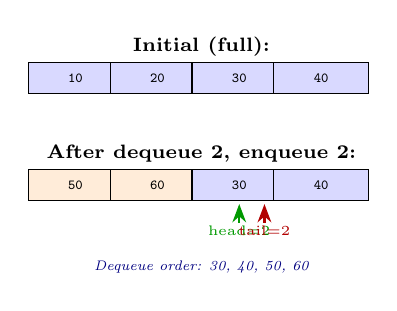
\begin{tikzpicture}[>=Stealth, scale=0.8]
  % State 1
  \node[font=\scriptsize\bfseries] at (2, 4.0) {Initial (full):};
  \foreach \i/\v in {0/10, 1/20, 2/30, 3/40} {
    \node[draw, minimum width=1.2cm, minimum height=0.4cm,
          fill=blue!15, font=\tiny\ttfamily] at (\i*1.3, 3.5) {\v};
  }

  % State 2
  \node[font=\scriptsize\bfseries] at (2, 2.3) {After dequeue 2, enqueue 2:};
  \foreach \i/\v/\c in {0/50/orange!15, 1/60/orange!15, 2/30/blue!15, 3/40/blue!15} {
    \node[draw, minimum width=1.2cm, minimum height=0.4cm,
          fill=\c, font=\tiny\ttfamily] at (\i*1.3, 1.8) {\v};
  }
  \draw[->, thick, green!60!black] (2*1.3, 1.2) -- (2*1.3, 1.5)
    node[below=0.15cm, font=\tiny] {head=2};
  \draw[->, thick, red!70!black] (2*1.3+0.4, 1.2) -- (2*1.3+0.4, 1.5)
    node[below=0.15cm, font=\tiny] {tail=2};

  % FIFO label
  \node[font=\tiny\itshape, text=blue!50!black] at (2, 0.5)
    {Dequeue order: 30, 40, 50, 60};
\end{tikzpicture}
\end{center}

\vspace{0.3em}
\begin{block}{Wraparound}
Tail wraps from index 3 back to index 0.
FIFO ordering is maintained through the
modulo arithmetic --- no data movement required.
\end{block}
\end{column}
\end{columns}
\end{frame}

% ===========================================================================
\section{Embedded Use Cases}
% ===========================================================================

\begin{frame}[fragile]{Use Case: Event Queue (ISR to Main Loop)}
\begin{columns}[T]
\begin{column}{0.52\textwidth}
\begin{lstlisting}[style=cstyle,
  title={ISR posts events, main loop dispatches}]
#include "tiku_kits_ds_queue.h"

/* Event IDs */
#define EVT_BUTTON_PRESS  1
#define EVT_TIMER_TICK    2
#define EVT_SENSOR_READY  3

static struct tiku_kits_ds_queue evt_q;

void event_init(void) {
    tiku_kits_ds_queue_init(&evt_q, 16);
}

/* Called from ISR context */
void event_post(int32_t evt_id) {
    /* Best-effort: drop if full */
    tiku_kits_ds_queue_enqueue(
        &evt_q, evt_id);
}

/* Called from main loop */
void event_dispatch(void) {
    tiku_kits_ds_elem_t evt;
    while (tiku_kits_ds_queue_dequeue(
               &evt_q, &evt)
           == TIKU_KITS_DS_OK) {
        switch (evt) {
        case EVT_BUTTON_PRESS:
            handle_button(); break;
        case EVT_TIMER_TICK:
            handle_timer();  break;
        case EVT_SENSOR_READY:
            handle_sensor(); break;
        }
    }
}
\end{lstlisting}
\end{column}

\begin{column}{0.44\textwidth}
\begin{center}
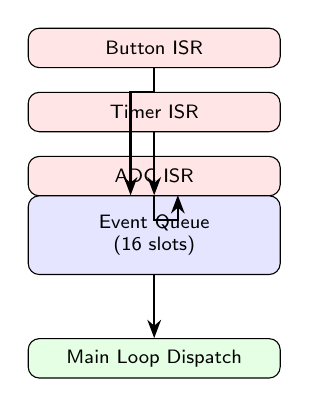
\begin{tikzpicture}[>=Stealth, node distance=0.4cm]
  \node[draw, rounded corners, fill=red!10,
        minimum width=3.2cm, minimum height=0.5cm,
        font=\scriptsize\sffamily] (btn) {Button ISR};
  \node[draw, rounded corners, fill=red!10,
        minimum width=3.2cm, minimum height=0.5cm,
        font=\scriptsize\sffamily, below=0.3cm of btn] (tmr) {Timer ISR};
  \node[draw, rounded corners, fill=red!10,
        minimum width=3.2cm, minimum height=0.5cm,
        font=\scriptsize\sffamily, below=0.3cm of tmr] (adc) {ADC ISR};

  \node[draw, rounded corners, fill=blue!10,
        minimum width=3.2cm, minimum height=1.0cm,
        font=\scriptsize\sffamily, below=0.8cm of tmr,
        align=center] (q)
    {Event Queue\\(16 slots)};

  \node[draw, rounded corners, fill=green!10,
        minimum width=3.2cm, minimum height=0.5cm,
        font=\scriptsize\sffamily, below=0.8cm of q] (main)
    {Main Loop Dispatch};

  \draw[->, thick] (btn.south) -- ++(0, -0.3) -| ([xshift=-0.3cm]q.north);
  \draw[->, thick] (tmr.south) -- (q.north);
  \draw[->, thick] (adc.south) -- ++(0, -0.3) -| ([xshift=0.3cm]q.north);
  \draw[->, thick] (q) -- (main);
\end{tikzpicture}
\end{center}

\vspace{0.3em}
\begin{block}{Pattern}
\begin{itemize}
  \item Multiple ISR producers
  \item Single main-loop consumer
  \item FIFO ensures fair ordering
  \item Queue depth limits burst size
\end{itemize}
\end{block}
\end{column}
\end{columns}
\end{frame}

% ---------------------------------------------------------------------------
\begin{frame}[fragile]{Use Case: Command Buffer and Message Passing}
\begin{columns}[T]
\begin{column}{0.48\textwidth}
\begin{lstlisting}[style=cstyle,
  title={Command buffer for serial protocol}]
#include "tiku_kits_ds_queue.h"

static struct tiku_kits_ds_queue cmd_q;

void cmd_init(void) {
    tiku_kits_ds_queue_init(&cmd_q, 8);
}

/* Parser queues parsed commands */
void cmd_submit(int32_t cmd_code) {
    if (tiku_kits_ds_queue_full(&cmd_q)) {
        /* Signal overflow to host */
        send_nack();
        return;
    }
    tiku_kits_ds_queue_enqueue(
        &cmd_q, cmd_code);
}

/* Executor processes in FIFO order */
void cmd_execute_next(void) {
    tiku_kits_ds_elem_t cmd;
    if (tiku_kits_ds_queue_dequeue(
            &cmd_q, &cmd)
        == TIKU_KITS_DS_OK) {
        execute(cmd);
    }
}
\end{lstlisting}
\end{column}

\begin{column}{0.48\textwidth}
\begin{lstlisting}[style=cstyle,
  title={Inter-task message passing}]
#include "tiku_kits_ds_queue.h"

/* Mailbox between two tasks */
static struct tiku_kits_ds_queue mailbox;

void mailbox_init(void) {
    tiku_kits_ds_queue_init(&mailbox, 8);
}

/* Task A sends a message */
int mailbox_send(int32_t msg) {
    return tiku_kits_ds_queue_enqueue(
        &mailbox, msg);
}

/* Task B receives a message */
int mailbox_recv(int32_t *msg) {
    return tiku_kits_ds_queue_dequeue(
        &mailbox, msg);
}

/* Task B checks if mail is waiting */
int mailbox_has_mail(void) {
    return !tiku_kits_ds_queue_empty(
        &mailbox);
}
\end{lstlisting}
\end{column}
\end{columns}
\end{frame}

% ===========================================================================
\section{Memory Layout}
% ===========================================================================

\begin{frame}{Memory Layout and Sizing}
\begin{columns}[T]
\begin{column}{0.48\textwidth}
\begin{center}
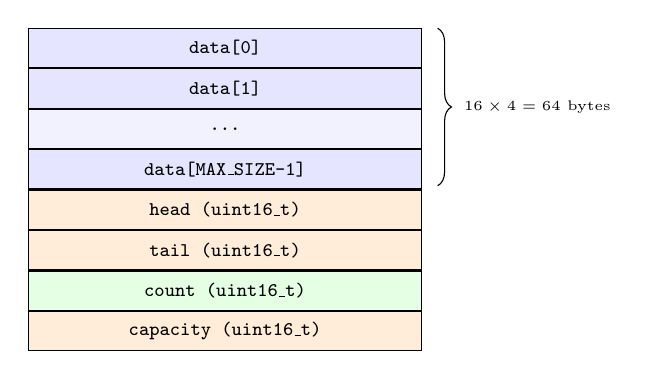
\begin{tikzpicture}[>=Stealth, node distance=0.0cm]
  \node[draw, minimum width=5cm, minimum height=0.5cm,
        fill=blue!10, font=\scriptsize\ttfamily] (d0) {data[0]};
  \node[draw, minimum width=5cm, minimum height=0.5cm,
        fill=blue!10, font=\scriptsize\ttfamily, below=0cm of d0] (d1) {data[1]};
  \node[draw, minimum width=5cm, minimum height=0.5cm,
        fill=blue!5, font=\scriptsize\ttfamily, below=0cm of d1] (d2) {...};
  \node[draw, minimum width=5cm, minimum height=0.5cm,
        fill=blue!10, font=\scriptsize\ttfamily, below=0cm of d2] (dn) {data[MAX\_SIZE-1]};
  \node[draw, minimum width=5cm, minimum height=0.5cm,
        fill=orange!15, font=\scriptsize\ttfamily, below=0cm of dn] (hd) {head (uint16\_t)};
  \node[draw, minimum width=5cm, minimum height=0.5cm,
        fill=orange!15, font=\scriptsize\ttfamily, below=0cm of hd] (tl) {tail (uint16\_t)};
  \node[draw, minimum width=5cm, minimum height=0.5cm,
        fill=green!10, font=\scriptsize\ttfamily, below=0cm of tl] (ct) {count (uint16\_t)};
  \node[draw, minimum width=5cm, minimum height=0.5cm,
        fill=orange!15, font=\scriptsize\ttfamily, below=0cm of ct] (cp) {capacity (uint16\_t)};

  \draw[decorate, decoration={brace, amplitude=5pt}]
    (2.7, 0.25) -- (2.7, -1.75)
    node[midway, right=6pt, font=\tiny] {$16 \times 4 = 64$ bytes};
\end{tikzpicture}
\end{center}
\end{column}

\begin{column}{0.48\textwidth}
\begin{block}{Size Formula}
\[
  \text{Total} = \texttt{MAX\_SIZE} \times \texttt{sizeof(elem\_t)} + 8
\]
\end{block}

\begin{table}
\centering
\scriptsize
\begin{tabular}{@{}rrr@{}}
\toprule
\textbf{MAX\_SIZE} & \textbf{elem\_t} & \textbf{Total (bytes)} \\
\midrule
4   & int32\_t & 24 \\
8   & int32\_t & 40 \\
16  & int32\_t & 72 \\
8   & int16\_t & 24 \\
16  & int16\_t & 40 \\
\bottomrule
\end{tabular}
\end{table}

\vspace{0.3em}
\begin{alertblock}{Default: 16 Slots}
The queue defaults to 16 elements --- sized for typical
event/command queues on embedded systems. Override
\texttt{TIKU\_KITS\_DS\_QUEUE\_MAX\_SIZE} for larger or smaller needs.
\end{alertblock}
\end{column}
\end{columns}
\end{frame}

% ===========================================================================
\section{Complexity}
% ===========================================================================

\begin{frame}{Time Complexity}
\begin{table}
\centering
\begin{tabular}{@{}lcc@{}}
\toprule
\textbf{Operation} & \textbf{Best Case} & \textbf{Worst Case} \\
\midrule
\texttt{init}     & $O(n)$ & $O(n)$ \\
\texttt{enqueue}  & $O(1)$ & $O(1)$ \\
\texttt{dequeue}  & $O(1)$ & $O(1)$ \\
\texttt{peek}     & $O(1)$ & $O(1)$ \\
\texttt{clear}    & $O(1)$ & $O(1)$ \\
\texttt{size}     & $O(1)$ & $O(1)$ \\
\texttt{full}     & $O(1)$ & $O(1)$ \\
\texttt{empty}    & $O(1)$ & $O(1)$ \\
\bottomrule
\end{tabular}
\end{table}

\vspace{0.5em}
\begin{block}{All Core Operations Are $O(1)$}
\begin{itemize}
  \item Modulo wrap replaces element shifting --- no memmove
  \item \texttt{init} is $O(n)$ due to \texttt{memset} zeroing the data array
  \item Constant, deterministic timing for every enqueue/dequeue
  \item Safe for ISR contexts where timing must be predictable
\end{itemize}
\end{block}
\end{frame}

% ===========================================================================
\section{Test Suite}
% ===========================================================================

\begin{frame}{Test Cases Overview}
\begin{table}
\centering
\small
\begin{tabular}{@{}clp{7cm}@{}}
\toprule
\textbf{\#} & \textbf{Test Function} & \textbf{What It Verifies} \\
\midrule
1 & \texttt{test\_kits\_ds\_queue\_init}
  & Initialization, capacity bounds, empty/full state \\
2 & \texttt{test\_kits\_ds\_queue\_enqueue\_dequeue}
  & Single enqueue/dequeue cycle, empty-dequeue error \\
3 & \texttt{test\_kits\_ds\_queue\_fifo\_order}
  & Enqueue 10,20,30; dequeue returns 10,20,30 \\
4 & \texttt{test\_kits\_ds\_queue\_peek}
  & Peek returns head, does not remove, updates after dequeue \\
5 & \texttt{test\_kits\_ds\_queue\_full\_empty}
  & Full/empty flags, enqueue-when-full error \\
6 & \texttt{test\_kits\_ds\_queue\_wraparound}
  & Head and tail wrap correctly, FIFO preserved \\
7 & \texttt{test\_kits\_ds\_queue\_size\_tracking}
  & Size increments/decrements, interleaved ops \\
8 & \texttt{test\_kits\_ds\_queue\_clear\_reset}
  & Clear resets state, dequeue after clear fails \\
9 & \texttt{test\_kits\_ds\_queue\_null\_inputs}
  & All functions reject NULL with ERR\_NULL; empty(NULL)=1 \\
\bottomrule
\end{tabular}
\end{table}
\end{frame}

% ===========================================================================
\section{Summary}
% ===========================================================================

\begin{frame}{Summary}
\begin{columns}[T]
\begin{column}{0.48\textwidth}
\begin{block}{What We Built}
\begin{itemize}
  \item Fixed-capacity FIFO queue
  \item 8 API functions: init, enqueue, dequeue, peek, clear, size, full, empty
  \item Ring-buffer based $O(1)$ enqueue/dequeue
  \item Count field --- no wasted slot
  \item Zero heap usage --- fully static
\end{itemize}
\end{block}

\begin{block}{Key Design Choices}
\begin{itemize}
  \item Application-level naming: enqueue/dequeue
  \item Separate count field for full/empty detection
  \item Default capacity 16 (sized for event queues)
  \item \texttt{empty(NULL)} returns 1 (safe default)
  \item NULL-pointer validation on all functions
\end{itemize}
\end{block}
\end{column}

\begin{column}{0.48\textwidth}
\begin{block}{Use Cases}
\begin{itemize}
  \item ISR-to-main-loop event queues
  \item Serial command buffers
  \item Inter-task message passing
  \item Debug log output buffering
  \item Task scheduling (round-robin)
\end{itemize}
\end{block}

\begin{block}{Files}
\scriptsize
\begin{tabular}{@{}lp{4.5cm}@{}}
Common: & \texttt{ds/tiku\_kits\_ds.h} \\
Header: & \texttt{ds/queue/tiku\_kits\_ds\_queue.h} \\
Source: & \texttt{ds/queue/tiku\_kits\_ds\_queue.c} \\
Tests:  & \texttt{tests/ds/test\_kits\_ds\_queue.c} \\
\end{tabular}
\end{block}
\end{column}
\end{columns}
\end{frame}

% ---------------------------------------------------------------------------
\begin{frame}{Thank You}
\begin{center}
\Large\textbf{TikuKits DS: Queue}\\[0.5em]
\normalsize FIFO Queue for Event-Driven Embedded Systems\\[1.5em]

\begin{tabular}{rl}
  Repository: & \url{https://github.com/tikuos/tikuOS} \\
  License:    & Apache 2.0 \\
  Common:     & \texttt{tikukits/ds/tiku\_kits\_ds.h} \\
  Header:     & \texttt{tikukits/ds/queue/tiku\_kits\_ds\_queue.h} \\
  Source:     & \texttt{tikukits/ds/queue/tiku\_kits\_ds\_queue.c} \\
  Tests:      & \texttt{tikukits/tests/ds/test\_kits\_ds\_queue.c} \\
\end{tabular}
\end{center}
\end{frame}

\end{document}
